\documentclass[conference]{IEEEtran}
\IEEEoverridecommandlockouts
\usepackage{cite}
\usepackage{amsmath,amssymb,amsfonts}
\usepackage{algorithm}
\usepackage{algpseudocode}
\usepackage{graphicx}
\usepackage{booktabs}
\usepackage{multirow}
\usepackage{xcolor}
\usepackage{tikz}
\usetikzlibrary{arrows.meta,positioning,fit,backgrounds}
\usepackage[hidelinks]{hyperref}
\graphicspath{{figures/}}
\newcommand{\fndbound}{2,436}
\newcommand{\fndfrac}{87.6}


\begin{document}

\title{QHP-Net: Quorum Sensing, Hippopotamus Optimisation and Pheromone-Learned Routing for Maximum-Lifetime Green Wireless Sensor Networks}

\author{\IEEEauthorblockN{Ashish Sharma\IEEEauthorrefmark{1}, Yogesh Sharma\IEEEauthorrefmark{1}, Satvik Rastogi\IEEEauthorrefmark{2}, Ansh Rai\IEEEauthorrefmark{2}, Lakshay Gupta\IEEEauthorrefmark{2}, Vansh Tomar\IEEEauthorrefmark{2}}
\IEEEauthorblockA{\IEEEauthorrefmark{1}Assistant Professor, \IEEEauthorrefmark{2}Student, Department of Computer Science and Engineering\\
Maharaja Agrasen Institute of Technology, Delhi, India\\
ashish@mait.ac.in, yogeshsharma@mait.ac.in, satvikrastogi777@gmail.com,\\ raiansh230405@gmail.com, lakshay22122004@gmail.com, vanshwar@gmail.com}}

\maketitle

\begin{abstract}
A wireless sensor network's lifetime is decided by three choices: which nodes may become cluster heads, which of them serve and who joins whom, and how heads reach the sink. We propose QHP-Net, which gives each choice its own bio-inspired mechanism, each aimed at a failure mode measured in our earlier nine-protocol study. Bacterial quorum sensing with a refractory term picks rested, locally strong candidates. Hippopotamus Optimisation selects heads by minimising the predicted bottleneck stress $\max_i \text{drain}_i/E_i$, and members join whichever head, or the sink directly, minimises their stress. An ant-pheromone link memory learns per-link delivery probability from ARQ acknowledgements alone and drives ETX-aware forwarding. We evaluated QHP-Net against eight protocols, including NSGA-II, the best full-yield protocol of the earlier study, and our earlier HIECF framework, in one engine with energy conservation asserted, over 30 paired topologies. On the lossy channel QHP-Net's first node dies at round 2,133, 249 rounds (13.2\%) after NSGA-II's and 43--52\% after the fuzzy, DQN and HIECF selectors. It wins in all 30 topologies (paired $t(29)=46.2$, $p_{Holm}<10^{-27}$, $d_z=8.4$, confirmed by Wilcoxon), delivers 98.3\% of readings at 16\% less energy per reading, and reaches \fndfrac\% of a physical upper bound. Its gain persists without packet loss (+168 rounds), under heterogeneous energy, with uplink costs charged, and across a nine-cell size sweep. An ablation shows that each selection and clustering mechanism contributes 42--328 rounds, that learned link quality is as good as the true link quality, and that a Physarum congestion router performs worse.
\end{abstract}

\begin{IEEEkeywords}
Wireless sensor networks, network lifetime, green networking, cluster-head selection, quorum sensing, hippopotamus optimization, ant colony, ETX routing, paired t-test, ablation study.
\end{IEEEkeywords}

%% ======================================================================
\section{Introduction}
%% ======================================================================
A sensor node spends most of its energy on its radio, and in most deployments its battery is never replaced, so the way a network organises its transmissions decides how long it lives~\cite{heinzelman2002leachc}. Clustering is the standard answer: members send short packets to a cluster head (CH), which fuses them and makes the one expensive transmission to the base station (BS)~\cite{heinzelman2000leach}. Three design decisions follow, and every protocol makes them, implicitly or explicitly: \emph{who may become a head} (candidacy), \emph{which candidates serve and who joins whom} (selection and clustering), and \emph{how heads reach the sink} (routing).

Our previous study rebuilt nine protocols from three methodological generations in one paired simulation engine~\cite{sharma2026unified}. Three of its measurements motivate this paper. (i) Among protocols that deliver every reading, the multi-objective NSGA-II selector~\cite{deb2002nsga2} had the latest first node death (FND); the reactive TEEN family lived longer only by suppressing about 89\% of the readings~\cite{manjeshwar2001teen}. (ii) Learned selectors concentrated the head duty on a few nodes (duty Gini up to 0.70), which is what killed them early. (iii) Clustering \emph{redistributes} lifetime rather than extending it: a member's reading is paid for twice in radio electronics, once to send and once to receive, so near the sink, clustering costs more than it saves. Our companion framework HIECF~\cite{sharma2026hiecf} combined type-2 fuzzy filtering, Q-learning and multi-hop routing, but was evaluated against behavioural models of its baselines rather than implementations, so its margins could not be tested for significance.

This paper proposes \textbf{QHP-Net}, which gives each of the three decisions its own bio-inspired mechanism, each aimed at one of those measured failure modes:
\begin{itemize}
\item \textbf{Candidacy by bacterial quorum sensing}~\cite{miller2001quorum}. Each node secretes an autoinducer in proportion to its energy, suppressed by a refractory term after it has served. A node becomes a candidate when its secretion exceeds the concentration around it. Candidates are therefore healthy, rested and spread over the field, which addresses duty concentration (ii).
\item \textbf{Selection and clustering by Hippopotamus Optimisation (HO)}~\cite{amiri2024hippo}, a recent swarm metaheuristic, minimising the predicted \emph{bottleneck stress} $\max_i \text{drain}_i/E_i$ rather than total energy, which is the max--min view of lifetime~\cite{chang2004maxlife}. Members join the head, \emph{or the sink directly}, that minimises their stress contribution. This yields unequal clusters and switches clustering off exactly where it does not pay (iii).
\item \textbf{Routing with an ant-pheromone link memory}~\cite{dorigo2006aco}. Link quality is never given to the protocol. Every ARQ attempt evaporates a link's trail and every acknowledgement deposits on it, so the trail converges to the per-attempt delivery probability, from which an ETX~\cite{decouto2003etx} is derived for stress-aware forwarding between heads.
\end{itemize}
We compare QHP-Net with eight protocols, including a faithful HIECF, in the same engine: 30 paired topologies on lossy and ideal channels, a 3$\times$3 node-count by field-size sweep, three-level heterogeneity and a stricter control-accounting setting. Comparisons use paired $t$-tests with Holm correction, effect sizes, normality checks and Wilcoxon confirmation, plus a seven-variant ablation. The parameters of QHP-Net were fixed on separate tuning seeds before any test run.

%% ======================================================================
\section{Recent Work}
%% ======================================================================
Swarm metaheuristics dominate recent CH selection. HHOCFR uses an improved Harris hawks optimiser for joint head selection and cluster formation, with fuzzy relay choice~\cite{jing2024hhocfr}. EECHIGWO~\cite{reddy2023eechigwo} and MOGWO~\cite{sennan2025mogwo} use grey-wolf variants with multi-term or fuzzy fitness. An improved sparrow search adds sine and Cauchy perturbations~\cite{wang2025issa}, and BSBOC applies a binary secretary-bird optimiser with a Voronoi term and is one of few to apply a Wilcoxon test~\cite{abdulkareem2025bsboc}. Hybrids pair optimisers or add learning: whale with tunicate swarm~\cite{singh2022wtsa}, bat with artificial bee colony for joint clustering and routing~\cite{mohammed2026baabc}, extended with multi-agent RL routing~\cite{mohammed2026marl}, WOA--GWO with DRL sleep scheduling~\cite{nareshkumar2026rlmhwo}, African vulture with Aquila optimisers~\cite{mathankumar2026avaqoa}, and quantum PSO with a dueling double DQN~\cite{liu2026qpsodrl}. Slime-mould ideas appear as the Slime Mould Algorithm for CH selection~\cite{belloula2026smawsn} and as Physarum-inspired routing~\cite{zhang2013pirp,li2011slimemold}. HO itself has been used for CH selection with a mobile sink~\cite{kaushal2025hoam}.

Table~\ref{tab:recent} sets the closest works against ours. Two gaps recur. Link loss is rarely modelled, so the cost of retransmissions on long sink hops, which our earlier study found decisive~\cite{sharma2026unified}, is invisible. Significance testing is rarely reported. To the best of our knowledge, from searches of Crossref, OpenAlex and Europe PMC, no WSN protocol combines bacterial quorum sensing for candidacy, a metaheuristic for selection and a learned pheromone link memory for routing.

\begin{table}[t]
\caption{Closest recent works. ``Loss'' = packet loss modelled; ``Test'' = significance test reported.}
\label{tab:recent}
\centering\footnotesize
\setlength{\tabcolsep}{2.5pt}
\begin{tabular}{@{}lllcc@{}}
\toprule
Work & CH selection & Routing & Loss & Test\\
\midrule
HHOCFR~\cite{jing2024hhocfr} & Improved HHO & Fuzzy relay CH & -- & --\\
MOGWO~\cite{sennan2025mogwo} & MO grey wolf & Single hop & -- & --\\
BSBOC~\cite{abdulkareem2025bsboc} & Secretary bird & Single hop & -- & Wilcoxon\\
MARL-BA-ABC~\cite{mohammed2026marl} & Bat + ABC & Multi-agent RL & partial & --\\
SMA-WSN~\cite{belloula2026smawsn} & Slime mould alg. & Per hop & failures & CI\\
HOAM~\cite{kaushal2025hoam} & Hippopotamus & Mobile sink & -- & --\\
\textbf{QHP-Net} & QS + HO & Pheromone ETX & \checkmark & paired $t$\\
\bottomrule
\end{tabular}
\end{table}

%% ======================================================================
\section{System Model}
%% ======================================================================
$N$ static nodes are placed uniformly in a $W\times W$ field with the BS outside it at $(W/2,1.5W)$; the headline case is $N{=}100$, $W{=}100$\,m, $E_0{=}1$\,J (Table~\ref{tab:params}). Every node senses one reading per round, carried in a $k{=}4000$-bit packet. Radio energy follows the first-order model~\cite{heinzelman2002leachc},
\begin{equation}
E_{tx}(k,d)=kE_{el}+\begin{cases}k\varepsilon_{fs}d^2, & d<d_0\\ k\varepsilon_{mp}d^4, & d\ge d_0\end{cases},\qquad E_{rx}(k)=kE_{el},
\label{eq:radio}
\end{equation}
with $d_0=\sqrt{\varepsilon_{fs}/\varepsilon_{mp}}=87.7$\,m and a fusion charge $E_{DA}$ per bit received. A head emits one fused packet regardless of how many it receives (ideal fusion). Packet loss comes from a link budget: log-distance path loss with exponent $n{=}3$ and a per-link shadowing term $X_{ij}\sim\mathcal N(0,4^2)$\,dB drawn once per topology~\cite{rappaport2002wireless}, non-coherent BFSK bit errors, and $\text{PER}_{ij}=1-(1-\text{BER}_{ij})^k$. Failed packets are retried up to twice, and every attempt pays full transmit and receive energy. Control packets are 200 bits. The engine prices them by protocol class: distributed protocols pay advertisement, join and TDMA schedule; centralised ones pay the schedule and the sink's downlink. Every non-head node that transmits receives a schedule every round, whether from its head or, if it is sink-bound, from the BS. A protocol returns only a structure (heads and next hops). It cannot write energy, and energy conservation is asserted to $10^{-9}$\,J in every run.

\begin{table}[t]
\caption{Simulation parameters (shared by all protocols)}
\label{tab:params}
\centering\footnotesize
\begin{tabular}{@{}ll@{\hspace{8pt}}ll@{}}
\toprule
$N$, field & 100, $100{\times}100$\,m & $E_{el}$ & 50\,nJ/bit\\
BS & (50, 150)\,m & $\varepsilon_{fs}$ & 10\,pJ/bit/m$^2$\\
$E_0$ & 1\,J & $\varepsilon_{mp}$ & 0.0013\,pJ/bit/m$^4$\\
Data / ctrl & 4000 / 200 bits & $E_{DA}$ & 5\,nJ/bit\\
Head fraction $p$ & 0.05 & $P_t$, $PL_{1m}$ & 12\,dBm, 40\,dB\\
Re-cluster & every 5 rounds & $n$, $\sigma$, noise & 3.0, 4\,dB, $-105$\,dBm\\
Round cap & 7000 & ARQ retries & 2\\
Paired runs & 30 per setting & Readings & Ornstein--Uhlenbeck\\
\bottomrule
\end{tabular}
\end{table}

%% ======================================================================
\section{Proposed QHP-Net}
%% ======================================================================
QHP-Net re-clusters every five rounds, and immediately if a head dies (Fig.~\ref{fig:arch}). The sink runs layers 2 and 3 from the state that candidates report. Let $E_i$ be the residual energy, $r_i^h$ the last round node $i$ served as head, and $k_h=\max(1,\text{round}(p\,N_{alive}))$ the head count shared by all protocols.

\begin{figure}[t]
\centering
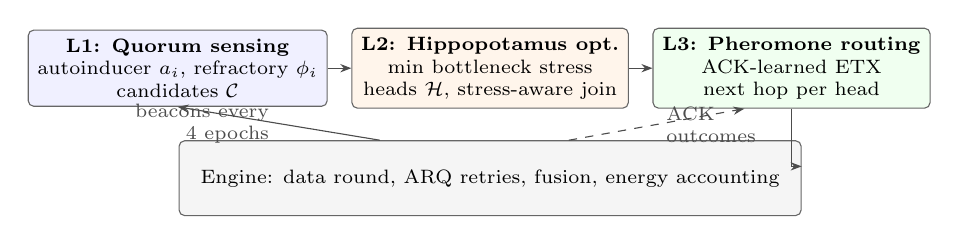
\begin{tikzpicture}[font=\scriptsize, node distance=3mm,
  box/.style={draw=black!60, rounded corners=2pt, align=center, minimum width=2.45cm, minimum height=0.95cm, fill=#1},
  box/.default=white, arr/.style={-{Stealth[length=4pt]}, black!70}]
\node[box=blue!6] (qs) {\textbf{L1: Quorum sensing}\\autoinducer $a_i$, refractory $\phi_i$\\candidates $\mathcal C$};
\node[box=orange!8, right=of qs] (ho) {\textbf{L2: Hippopotamus opt.}\\min bottleneck stress\\heads $\mathcal H$, stress-aware join};
\node[box=green!6, right=of ho] (ph) {\textbf{L3: Pheromone routing}\\ACK-learned ETX\\next hop per head};
\node[box=black!4, below=4mm of ho, minimum width=7.9cm] (eng) {Engine: data round, ARQ retries, fusion, energy accounting};
\draw[arr] (qs) -- (ho); \draw[arr] (ho) -- (ph);
\draw[arr] (ph.south) |- ([yshift=1.5mm]eng.east);
\draw[arr] ([xshift=-14mm]eng.north) -- node[left,align=right]{beacons every\\4 epochs} ([xshift=0mm]qs.south);
\draw[arr, dashed] ([xshift=10mm]eng.north) -- node[right,align=left]{ACK\\outcomes} ([xshift=-6mm]ph.south);
\end{tikzpicture}
\caption{QHP-Net. Each layer uses a different bio-inspired mechanism. Dashed: per-round ACK feedback used to learn link pheromone.}
\label{fig:arch}
\end{figure}

\subsection{Layer 1: Quorum-Sensing Candidacy}
Every node secretes an autoinducer
\begin{equation}
a_i=\frac{E_i}{\bar E_0}\,(1-\phi_i),\qquad \phi_i=e^{-(r-r_i^h)/\tau},
\label{eq:secretion}
\end{equation}
where $\phi_i$ is a refractory term that silences a node that has just served ($\phi_i=0$ if it never has). Neighbours within the density radius $\rho$ exchange $a_i$ in one beacon. Each node computes, from the beacons it hears and nothing else, the kernel-weighted concentration and its quorum ratio,
\begin{equation}
C_i=\frac{\sum_j K_{ij}a_j}{\sum_j K_{ij}},\quad K_{ij}=e^{-d_{ij}^2/2\rho^2}\mathbb 1[d_{ij}<\rho],\quad q_i=\frac{a_i}{C_i}.
\label{eq:quorum}
\end{equation}
A node with $q_i\ge1$ out-secretes its neighbourhood and expresses the candidate phenotype. The pool is the top $n_c$ nodes by $q_i(1-\phi_i)$, with $n_c=\text{clip}(|\{q_i\ge1\}|,3k_h,8k_h)$. Because $q_i$ is \emph{relative}, every region of the field contributes candidates even late in life. Beacons are sent every four epochs and are charged as real control packets. Between beacons the sink, which assigned past heads, applies the refractory factor itself. As for every centralised protocol here, node state reaches the sink on data traffic~\cite{sharma2026unified}. On top of that, QHP-Net pays an explicit 200-bit report from each candidate, and Section~\ref{sec:robust} charges every centralised protocol's uplink.

\subsection{Layer 2: Hippopotamus-Optimised Selection and Clustering}
\emph{Stress model.} For a head set $\mathcal H$, let $\text{ETX}_{ij}=1+\hat p_{ij}+\hat p_{ij}^2$ be the expected number of attempts (at most three) under the learned loss estimate $\hat p_{ij}$ (Layer 3), with $c_{ij}=\text{ETX}_{ij}E_{tx}(k,d_{ij})$ and $\hat c_{ij}=\text{ETX}_{ij}(E_{rx}(k)+kE_{DA})$. Each alive non-head node joins
\begin{equation}
h^\star(i)=\arg\min_{h\in\mathcal H\cup\{\text{BS}\}}\;\sigma_{ih},\quad \sigma_{ih}=\frac{c_{ih}}{E_i}+\frac{\hat c_{ih}}{E_h},\ \ \sigma_{i\,\text{BS}}=\frac{c_{i\,\text{BS}}}{E_i},
\label{eq:join}
\end{equation}
i.e., it charges each joule to the battery that pays it. Clusters therefore shrink around weak heads (unequal clustering), and nodes for which the second reception costs more than the sink hop transmit directly (the \emph{direct regime}). Summing transmissions and receptions gives the predicted per-round drain $D_i(\mathcal H)$, and the fitness is
\begin{equation}
F(\mathcal H)=\max_i\frac{D_i}{E_i}+\mu\,\frac{1}{N_{alive}}\sum_i\frac{D_i}{E_i},
\label{eq:fitness}
\end{equation}
whose first term is the reciprocal of the predicted time to the next death~\cite{chang2004maxlife}.

\emph{Search.} A herd of $P{=}20$ hippopotamuses encodes $k_h$ points in the field; each point decodes to the nearest unused candidate. HO~\cite{amiri2024hippo} iterates three phases for $T{=}25$ iterations, with greedy acceptance. In the river phase (exploration), males move toward the dominant hippo, $X_i'=X_i+y_1(D_{hippo}-I_1X_i)$, and immature hippos toward or away from a random group mean $MG_i$ depending on $e^{-t/T}$. In the predator-defence phase, $X_i'=RL\odot X_{pred}+\frac{b}{c-d\cos 2\pi g}\cdot\frac{1}{\delta_i}$, with a Lévy vector $RL$~\cite{mantegna1994levy} and predator distance $\delta_i$. In the escape phase (exploitation), $X_i'=X_i+r(\frac{lb}{t}+s_1(\frac{ub}{t}-\frac{lb}{t}))$, a shrinking local search. The herd is seeded with the top-$k_h$ quorum candidates and with the previous epoch's best (elitist memory).

\subsection{Layer 3: Pheromone-Learned Routing}
Each node keeps a pheromone $\tau_{ij}\in(0,1]$ per link, initialised to 1: the protocol is given no channel model, no path-loss parameters and no knowledge of whether the channel is lossy. After each data packet with $n$ attempts,
\begin{equation}
\tau_{ij}\leftarrow\tau_{ij}(1-\varrho)^{n}+\varrho\,\mathbb 1[\text{acked}],\qquad \hat p_{ij}=1-\tau_{ij},
\label{eq:pheromone}
\end{equation}
which is the ant-colony evaporate-and-deposit rule~\cite{dorigo2006aco} applied to delivery. Its fixed point is the per-attempt success probability, learned from acknowledgements the sender already receives; links are reciprocal. A head forwards to $\arg\min_{j}\sigma_{hj}$ over the BS and the heads strictly closer to the BS, which makes routes acyclic. With ideal fusion a head's packet costs exactly one hop, since every downstream head transmits anyway, so the per-hop stress $\sigma_{hj}$ is the exact marginal cost. The same rule is used inside $F$, so the optimiser and the deployed routes agree.

Algorithm~\ref{alg:qhp} summarises one epoch. Its cost is $O(N\rho^2)$ for quorum sensing and $O(PT\,N k_h)$ for the search, vectorised at the sink.

\begin{algorithm}[t]
\caption{QHP-Net epoch (every 5 rounds or on head death)}
\label{alg:qhp}
\footnotesize
\begin{algorithmic}[1]
\Require residual energies $E$, head history $r^h$, pheromone $\tau$
\State $\hat p\gets 1-\tau$;\ \ $\text{ETX}\gets 1+\hat p+\hat p^2$ \Comment{L3 memory}
\If{beacon epoch} each node broadcasts $a_i$ (Eq.~\ref{eq:secretion}); compute $q_i$ (Eq.~\ref{eq:quorum}) \EndIf
\State $\mathcal C\gets$ top-$n_c$ nodes by $q_i(1-\phi_i)$; candidates report state \Comment{L1}
\State initialise herd $X\in[0,W]^{P\times k_h\times2}$; seed with top-$k_h$ of $\mathcal C$ and last best
\For{$t=1\ldots T$} \Comment{L2: HO}
  \State river phase (males $\to D_{hippo}$; immatures $\to/\leftarrow MG$); greedy accept
  \State predator defence with Lévy flight; greedy accept
  \State escape inside bounds $[lb/t,ub/t]$; greedy accept
\EndFor
\State $\mathcal H\gets$ decode$(X_{best})$; heads route to $\arg\min_j\sigma_{hj}$ \Comment{L3}
\State members join $h^\star(i)$ or the BS (Eq.~\ref{eq:join})
\For{each round of the epoch} transmit; update $\tau$ from ACKs (Eq.~\ref{eq:pheromone}) \EndFor
\end{algorithmic}
\end{algorithm}

%% ======================================================================
\section{Experimental Design}
%% ======================================================================
\emph{Protocols.} Direct transmission, LEACH~\cite{heinzelman2000leach}, PEGASIS~\cite{lindsey2002pegasis}, TEEN~\cite{manjeshwar2001teen}, NSGA-II (population 40, 30 generations, three objectives)~\cite{deb2002nsga2}, an interval type-2 fuzzy selector with 27 rules and Karnik--Mendel reduction~\cite{karnik1999type2,karnik2001centroid}, a $4{\to}16{\to}2$ DQN~\cite{mnih2015dqn} trained offline on 40 disjoint seeds and then frozen, HIECF~\cite{sharma2026hiecf} (type-2 fuzzy filter, tabular Q-learning, $d^2/E$ multi-hop routing), and QHP-Net. All share the engine and $k_h$. NSGA-II and QHP-Net re-optimise every 5 rounds or on a head death. LEACH, TEEN, Fuzzy-T2, DQN and HIECF re-cluster every round, their native behaviour and the setting of~\cite{sharma2026unified}. QHP-Net warm-starts its search from the previous epoch, so we also ran NSGA-II with the same warm start as a fairness check.

\emph{Pairing and seeds.} Seed $i$ fixes the positions, energies, shadowing matrix and readings, so all protocols at index $i$ face an identical world. Test seeds are $0$--$29$. QHP-Net's parameters ($\tau{=}20$, $\mu{=}0.5$, $\varrho{=}0.1$, $P{=}20$, $T{=}25$, beacon period 4) were chosen on seeds $500$--$505$ only. Every setting is run with packet loss and on an ideal channel.

\emph{Metrics.} FND, HND and LND (the round of the first, half and last death; censored at 7000), the area under the alive-node curve (AUC), data yield (readings delivered over readings taken), energy per delivered reading (green metric), duty Gini and setup time.

\emph{Statistics.} For each metric we form 30 per-seed differences $\Delta_i=x_i^{\text{QHP}}-x_i^{\text{opp}}$ and apply a two-sided paired $t$-test. We report the mean difference, its 95\% $t$-interval, Cohen's $d_z=\bar\Delta/s_\Delta$~\cite{cohen1988power}, Holm-corrected $p$ across opponents~\cite{holm1979simple}, a Shapiro--Wilk test of normality on $\Delta$~\cite{shapiro1965analysis}, and the Wilcoxon signed-rank $p$~\cite{wilcoxon1945individual,demsar2006statistical} as a distribution-free check.

%% ======================================================================
\section{Previous Study and the Opponent}
%% ======================================================================
Table~\ref{tab:prev} places the first-death results of our previous nine-protocol study~\cite{sharma2026unified} next to the same protocols rerun in this engine, which reimplements its harness from the parameters alone. Every mean is within 5\% of the earlier value. The largest gaps are TEEN ($+4.0\%$) and DQN ($-4.7\%$), and the DQN was retrained here. The reproduction is close enough that the opponent can be chosen on the earlier evidence. TEEN has the latest FND in both studies, but it reaches it by delivering only about 11\% of the readings. Among protocols that deliver what they sense, NSGA-II had the latest FND, significantly ahead of LEACH by 827 rounds ($p_{Holm}{=}0.0004$), so \textbf{NSGA-II is the primary opponent of the paired $t$-test}. TEEN is kept as a reference and HIECF as our own earlier design.

\begin{table}[t]
\caption{First node death (rounds, lossy channel): previous study~\cite{sharma2026unified} vs.\ this engine, 30 paired runs each}
\label{tab:prev}
\centering\footnotesize
\begin{tabular}{@{}lrrr@{}}
\toprule
Protocol & Previous study & This engine & Yield (this)\\
\midrule
Direct & 114 & 115 & 0.967\\
LEACH & 1,046 & 1,051 & 0.867\\
PEGASIS & 1,588 & 1,600 & 0.827\\
TEEN & 2,208 & 2,297 & 0.107\\
NSGA-II & \textbf{1,873} & \textbf{1,884} & 0.888\\
Fuzzy-T2 & 1,462 & 1,476 & 0.899\\
DQN & 1,472 & 1,403 & 0.882\\
\bottomrule
\end{tabular}
\end{table}

%% ======================================================================
\section{Simulation Results}
%% ======================================================================
\subsection{Lifetime, Delivery and Energy}
Table~\ref{tab:life} and Fig.~\ref{fig:alive} give the lossy-channel results. QHP-Net's first death comes at round $2{,}133\pm19$: 249 rounds (13.2\%) after NSGA-II, 43--52\% after the fuzzy, DQN and HIECF selectors, and 2.0$\times$ after LEACH. Its FND standard deviation is 0.58 of NSGA-II's and one fifteenth of PEGASIS's. Only TEEN dies later, and only because it suppresses 89\% of the readings.

QHP-Net delivers 98.3\% of the readings it senses, the highest yield of any clustered protocol, and spends 0.470\,mJ per delivered reading, 16\% less than the cheapest baseline (PEGASIS and NSGA-II, 0.56\,mJ). It lives longer \emph{and} delivers more data per joule, which is the green-network result. Retransmissions take 0.2\% of its budget, against 3.6\% for NSGA-II and 5.3\% for LEACH, because the learned ETX keeps sink hops out of the packet-error waterfall. This holds although it pays the largest control share of the centralised protocols (5.3\%).

Max--min balancing has a cost. Nodes run down together, so HND follows FND by only 32 rounds and the last node dies at round 2,208, before NSGA-II (2,397), DQN (2,477), PEGASIS (2,560) and Direct (3,186). For coverage, keeping every node alive to round 2,133 is worth more than keeping a few to round 2,500. On the area under the alive curve, which counts both, QHP-Net ties PEGASIS ($216.4$ vs.\ $216.2\times10^3$, n.s.) and beats every other full-yield protocol, NSGA-II by $15.4\times10^3$.

\emph{Upper bound.} Until the first death every reading must leave its node each round, costing at least one transmission plus either the sink amplifier or a reception and fusion elsewhere. Summing this floor, with no control, retries or relaying, bounds FND at \fndbound{} rounds on average; QHP-Net reaches \fndfrac\% of it.

\begin{table}[t]
\caption{Lifetime on the lossy channel, mean $\pm$ s.d.\ over 30 paired runs. AUC in $10^3$ node-rounds; mJ per delivered reading. $^c$\,censored at the 7000-round cap in every run.}
\label{tab:life}
\centering\footnotesize
\setlength{\tabcolsep}{2.6pt}
\begin{tabular}{@{}lrrrrrr@{}}
\toprule
Protocol & FND & HND & LND & AUC & Yield & mJ/rd\\
\midrule
Direct & 115 $\pm$ 10 & 1,140 $\pm$ 200 & 3,186 $\pm$ 83 & 132.6 & 0.967 & 0.78 \\
LEACH & 1,051 $\pm$ 51 & 1,674 $\pm$ 28 & 2,160 $\pm$ 43 & 166.4 & 0.867 & 0.69 \\
PEGASIS & 1,600 $\pm$ 286 & 2,202 $\pm$ 9 & 2,560 $\pm$ 290 & 216.2 & 0.827 & 0.56 \\
TEEN & 2,297 $\pm$ 145 & 5,975 $\pm$ 223 & $>$7,000$^c$ & 558.9 & 0.107 & 1.65 \\
NSGA-II & 1,884 $\pm$ 33 & 1,984 $\pm$ 28 & 2,397 $\pm$ 151 & 201.1 & 0.888 & 0.56 \\
Fuzzy-T2 & 1,476 $\pm$ 61 & 1,922 $\pm$ 28 & 2,208 $\pm$ 52 & 189.2 & 0.899 & 0.59 \\
DQN & 1,403 $\pm$ 52 & 1,875 $\pm$ 31 & 2,477 $\pm$ 79 & 189.0 & 0.882 & 0.60 \\
HIECF & 1,490 $\pm$ 128 & 1,930 $\pm$ 44 & 2,218 $\pm$ 66 & 191.2 & 0.905 & 0.58 \\
\textbf{QHP-Net} & 2,133 $\pm$ 19 & 2,165 $\pm$ 17 & 2,208 $\pm$ 27 & 216.4 & 0.983 & 0.47 \\

\bottomrule
\end{tabular}
\end{table}

\begin{figure*}[t]
\centering
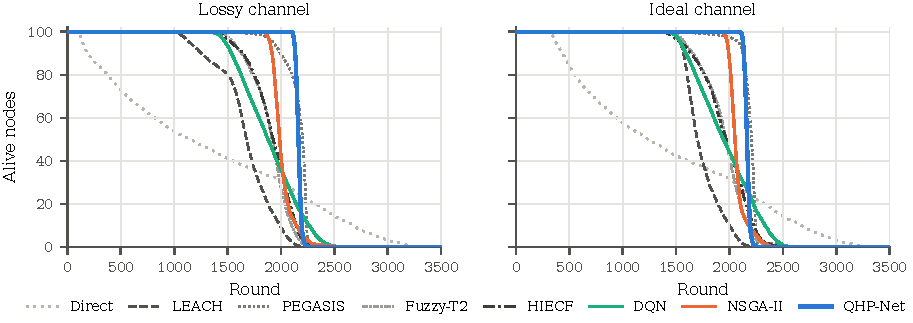
\includegraphics[width=0.94\textwidth]{alive}
\caption{Alive nodes per round, mean of 30 paired topologies (TEEN, censored at 7000 rounds, is omitted). QHP-Net keeps all 100 nodes alive longest under both channel models, and its curve does not move when packet loss is removed.}
\label{fig:alive}
\end{figure*}

\subsection{Paired $t$-Tests}
Table~\ref{tab:ttest} tests the per-topology differences. QHP-Net's first death is later than that of every full-yield opponent in \emph{all} 30 topologies on both channels; its smallest single margin over NSGA-II is 198 rounds (lossy) and 137 (ideal). Against NSGA-II the mean FND gain is $+249$ rounds, 95\% CI $[+238,+260]$, $t(29)=46.2$, $p_{Holm}=4.3\times10^{-28}$, $d_z=8.4$. The AUC gain is $15.4\times10^3$ node-rounds ($t(29)=38.0$, $d_z=6.9$). Shapiro--Wilk does not reject normality for NSGA-II ($p{=}0.23$) but does for some pairs (PEGASIS FND, $p{=}0.001$), so every cell was confirmed with the Wilcoxon test. All cells but one are significant under both tests after Holm correction ($p\le1.0\times10^{-5}$).

In our earlier study the FND gains of the fuzzy and DQN selectors over LEACH (417 and 426 rounds) shrank to an insignificant 17 and 22 on an ideal channel~\cite{sharma2026unified}. QHP-Net's gain does not vanish: without loss it still leads NSGA-II by 168 rounds ($d_z=8.6$) and every other full-yield protocol by 478--1,806. Its own FND is 2,133 on both channels, so its advantage comes from where energy is drawn, not only from avoiding loss. PEGASIS is the one opponent it does not beat on every metric: they tie on AUC under loss, and PEGASIS leads by $2.7\times10^3$ node-rounds on the ideal channel and reaches HND 37 rounds later. In exchange QHP-Net delivers 15.6 points more readings and its first node dies 533 rounds later.

\begin{table*}[t]
\caption{Paired differences QHP-Net $-$ opponent over 30 topologies: mean [95\% CI] and Cohen's $d_z$. Unless marked $^{ns}$, the difference is significant under both the paired $t$-test and the Wilcoxon test after Holm correction across opponents ($p\le1.0\times10^{-5}$). AUC in $10^3$ node-rounds. TEEN reaches its lead by delivering 11\% of the readings.}
\label{tab:ttest}
\centering\footnotesize
\begin{tabular}{@{}lrrrrrrrr@{}}
\toprule
& \multicolumn{2}{c}{$\Delta$FND, lossy} & \multicolumn{2}{c}{$\Delta$FND, ideal} & \multicolumn{2}{c}{$\Delta$AUC, lossy} & \multicolumn{2}{c}{$\Delta$AUC, ideal}\\
\cmidrule(lr){2-3}\cmidrule(lr){4-5}\cmidrule(lr){6-7}\cmidrule(l){8-9}
Opponent & mean [95\% CI] & $d_z$ & mean [95\% CI] & $d_z$ & mean & $d_z$ & mean & $d_z$\\
\midrule
LEACH & +1,082 [+1,062, +1,101] & 20.8 & +652 [+641, +662] & 23.0 & +50.0 & 19.9 & +42.2 & 24.9 \\
PEGASIS & +533 [+425, +641] & 1.8 & +478 [+362, +594] & 1.5 & +0.3$^{ns}$ & 0.1 & -2.7 & -1.4 \\
TEEN & -164 [-216, -111] & -1.2 & -2,154 [-2,207, -2,100] & -15.1 & -342.5 & -25.0 & -376.8 & -42.5 \\
NSGA-II & +249 [+238, +260] & 8.4 & +168 [+161, +175] & 8.6 & +15.4 & 6.9 & +9.5 & 6.6 \\
Fuzzy-T2 & +658 [+634, +682] & 10.3 & +632 [+609, +655] & 10.2 & +27.2 & 10.2 & +22.3 & 9.6 \\
DQN & +730 [+710, +750] & 13.6 & +657 [+648, +666] & 26.8 & +27.5 & 10.9 & +20.9 & 12.2 \\
HIECF & +643 [+595, +692] & 5.0 & +648 [+606, +690] & 5.7 & +25.3 & 8.3 & +21.0 & 7.9 \\

\bottomrule
\end{tabular}
\end{table*}





%%ABLATION%%


\bibliographystyle{IEEEtran}
\bibliography{refs}

\end{document}
